\documentclass{article}

\usepackage{arxiv}

\usepackage[utf8]{inputenc} % allow utf-8 input
\usepackage[T1]{fontenc}    % use 8-bit T1 fonts
\usepackage{lmodern}        % https://github.com/rstudio/rticles/issues/343
\usepackage{hyperref}       % hyperlinks
\usepackage{url}            % simple URL typesetting
\usepackage{booktabs}       % professional-quality tables
\usepackage{amsfonts}       % blackboard math symbols
\usepackage{nicefrac}       % compact symbols for 1/2, etc.
\usepackage{microtype}      % microtypography
\usepackage{graphicx}

\title{They're Clutching up! Team Momentum in Round-Based Esports}

\author{
    Tony ElHabr
   \\
     \\
   \\
  \texttt{\href{mailto:anthonyelhabr@gmail.com}{\nolinkurl{anthonyelhabr@gmail.com}}} \\
  }


% tightlist command for lists without linebreak
\providecommand{\tightlist}{%
  \setlength{\itemsep}{0pt}\setlength{\parskip}{0pt}}


% Pandoc citation processing
\newlength{\cslhangindent}
\setlength{\cslhangindent}{1.5em}
\newlength{\csllabelwidth}
\setlength{\csllabelwidth}{3em}
\newlength{\cslentryspacingunit} % times entry-spacing
\setlength{\cslentryspacingunit}{\parskip}
% for Pandoc 2.8 to 2.10.1
\newenvironment{cslreferences}%
  {}%
  {\par}
% For Pandoc 2.11+
\newenvironment{CSLReferences}[2] % #1 hanging-ident, #2 entry spacing
 {% don't indent paragraphs
  \setlength{\parindent}{0pt}
  % turn on hanging indent if param 1 is 1
  \ifodd #1
  \let\oldpar\par
  \def\par{\hangindent=\cslhangindent\oldpar}
  \fi
  % set entry spacing
  \setlength{\parskip}{#2\cslentryspacingunit}
 }%
 {}
\usepackage{calc}
\newcommand{\CSLBlock}[1]{#1\hfill\break}
\newcommand{\CSLLeftMargin}[1]{\parbox[t]{\csllabelwidth}{#1}}
\newcommand{\CSLRightInline}[1]{\parbox[t]{\linewidth - \csllabelwidth}{#1}\break}
\newcommand{\CSLIndent}[1]{\hspace{\cslhangindent}#1}

\usepackage{longtable}
\usepackage{amsmath}
\begin{document}
\maketitle


\begin{abstract}
My research investigates patterns in round win percentages in
professional Search and Destroy (SnD) matches of the popular
first-person shooter game Call of Duty (CoD). First, I find evidence
supprting the hypothesis that round win probability can be modeled as a
constant across the series, although not at the naive 50\%. Second, I
examine post-streak round win probability, in search of evidence
positive recency (the ``hot hand'' fallacy) or negative recency (the
``gambler's falacy''). I find that teams perform significantly worse
than expected after streaks of 2, 3, and 4 wins when series end up going
to 9, 10, or 11 (maximum) rounds, suggesting the presence of negative
recency.
\end{abstract}


\hypertarget{introduction}{%
\section{Introduction}\label{introduction}}

\hypertarget{description-of-call-of-duty-search-and-destroy}{%
\subsection{Description of Call of Duty Search and
Destroy}\label{description-of-call-of-duty-search-and-destroy}}

Call of Duty (CoD), first released in 2003, is one of the most popular
first-person shooter (FPS) video game franchises of all-time. The most
popular mode in the competitive scene is ``Search and Destroy''
(SnD).\footnote{SnD bears resemblance to ``Bomb Defusal'' in
  Counter-Strike and ``Plant/Defuse'' in Valorant, two other FPS games
  played in more popular professional leagues.} SnD is a one-sided game
mode in which one team, the offensive side, tries to destroy one of two
designated bomb sites on the map.

In professional CoD SnD, a team take turns playing offense and defense
every round. They must win six rounds to win the series.\footnote{A
  maximum of 11 even rounds can be played. There is no ``sudden death''
  or ``win by two'' rule like there are for SnD equivalent in
  professional Counter-Strike and Valorant matches.} A round can end in
one of five ways:

\begin{enumerate}
\def\labelenumi{\arabic{enumi}.}
\tightlist
\item
  One team eliminates all members of the other team prior to a bomb
  plant. (Eliminating team wins.)
\item
  The offensive team eliminates all members of the defensive team after
  a bomb plant.\footnote{\begin{itemize}
    \tightlist
    \item
      The bomb can be picked up by any member of the offensive team.
    \item
      The bomb carrier is not obstructed at all by carrying the bomb
      (i.e.~movement is the same, weapon usage is the same).
    \item
      The defense does not get any visual indication for who is carrying
      the bomb.
    \item
      A bomb plant takes five seconds. The timer resets if the player
      stops planting site prior to completing it.
    \item
      A bomb defuse takes seven seconds. The timer resets if the player
      ``drops'' the bomb.
    \item
      The bomb takes 45 seconds to defuse after being planted.
    \end{itemize}} (Offense wins.)
\item
  The defensive team defuses the bomb after a bomb plant.\footnote{Often
    the defensive team will try to eliminate all team members prior to
    making the defuse, but in some cases, they may try to ``ninja''
    defuse.} (Defense wins.)
\item
  The offensive team does not make a plant by the time the round timer
  ends. (Defense wins.)
\end{enumerate}

I adopt the terminology ``series'' to refer to what CoD SnD players
typically call a ``match'', so as to emulate the terminology of playoff
series in professional leagues like the National Basketball Association,
National Hockey League, and Major League Baseball. A ``game'' or a
``match'' in such leagues is analogous to a ``round'' of CoD SnD.

\hypertarget{data}{%
\subsection{Data}\label{data}}

CoD has roughly gone through three eras of professional gaming: (1)
Major League Gaming (MLG) tournaments prior to 2016; (2) the CoD World
League (CWL), initiated in 2016; and (3) the 12-franchise CoD League
(CDL), operating since 2020. The CDL has completed three year-long
``seasons'' as of August 2022.\footnote{CoD is fairly unique compared to
  other esports in that it runs on an annual lifecycle (released coming
  in the late fall), where a new game is published every year under the
  same title. Each new game bears resemblance to past ones, often
  introducing relatively small variations (``improvements'') to
  graphics, game modes, and other facets of gameplay. During the CDL
  era, the games released have been Modern Warfare (2020), Cold War
  (2021) and Vanguard (2022).}

The data set consists of all SnD matches played in tournanaments and
qualifiers during the CDL era, totaling 7,792 rounds across 852 series.
Data was collected in spreadsheets by community member
``IOUTurtle''.\footnote{Data: \url{https://linktr.ee/CDLArchive}.
  Author: \url{https://twitter.com/IOUTurtle}}

The empirical offensive round win percentage across all rounds is
47.8\%.\footnote{Offensive round win percentage has been nearly constant
  across the three games during the CDL era: 1. 47.2\% in MW (2020) 2.
  47.9\% in Cold War (2021) 3. 48.1\% in Vanguard (2022)} Table
\ref{tbl:cod-o-win-prop-by-series-state} shows round win percentages by
series ``state'' (i.e.~the number of round wins by each team prior to an
upcoming round). Offensive round win rate is not quite constant,
although never veers more than 10\% from this global average.

\begin{longtable}{crrrrrr}
\caption{Offensive round win rates for the upcoming round, given both the offensive and defensive team's prior number of round wins}\label{tbl:cod-o-win-prop-by-series-state} \\
\toprule
& \multicolumn{6}{c}{Offense round wins} \\ 
\cmidrule(lr){2-7}
Defense round wins & 0 & 1 & 2 & 3 & 4 & 5 \\ 
\midrule
0 & 47.8\%
(852) & 46.6\%
(408) & 43.1\%
(216) & 43.5\%
(115) & 43.3\%
(67) & 40.5\%
(37) \\ 
1 & 48.6\%
(444) & 49.3\%
(418) & 51.5\%
(309) & 43.4\%
(205) & 43.3\%
(120) & 39.4\%
(99) \\ 
2 & 52.8\%
(218) & 48.9\%
(305) & 48.9\%
(315) & 46.6\%
(262) & 48.7\%
(189) & 42.1\%
(133) \\ 
3 & 54.5\%
(123) & 46.0\%
(200) & 49.6\%
(250) & 45.6\%
(248) & 44.4\%
(214) & 44.8\%
(174) \\ 
4 & 56.9\%
(65) & 54.5\%
(145) & 47.2\%
(193) & 44.7\%
(228) & 55.2\%
(221) & 50.5\%
(208) \\ 
5 & 47.4\%
(38) & 49.4\%
(83) & 47.1\%
(136) & 50.9\%
(175) & 45.2\%
(177) & 46.0\%
(202) \\ 
\bottomrule
\end{longtable}

\hypertarget{literature-review}{%
\section{Literature review}\label{literature-review}}

There have been a handful of studies of the distribution of games played
in a series of a professional sport. Most assume a constant probability
\(\phi\) of a given team winning a game in the series, regardless of the
series state. Mosteller (1952) observed that the American League had
dominated the National League in Major League Baseball's (MLB) World
Series matchups, implying that matchups should not modeled with
\(\phi = 0.5\). Mosteller proposed three approaches for identifying the
optimal constant probability value of the stronger team in the World
Series, finding \(\phi \approx 0.65\). in each case: (1) solving for
\(p\) from the empirical average number of games won by the loser of the
series, which he called the ``method of moments'' approach; (2)
maximizing the likelihood that the sample would have been drawn from a
population in which the probability of a team winning a game is constant
across the series (i.e.~maximum likelihood), and (3) minimizing the
chi-square goodness of fit statistic for \(\phi\).

Chance (2020) re-examines the constant probability notion in Major
League Baseball's (MLB) World Series (1923--2018), the National
Basketball Association's (NBA) Finals (1951--2018), and the National
Hockey League's (NHL) Stanley Cup (1939--2018). Chance finds strong
evidence against the null hypothesis of \(\phi = 0.5\) in the MLB and
NHL championship series when applying Mosteller's first and second
methods. Chance goes on to outline a conditional probability framework
(likelihood of winning a game given the series state) which can exactly
explain the distribution of the number of games played.

Momentum, one of most discussed topics in sports analytics, goes
hand-in-hand with a discussion of the nature of series
outcomes.\footnote{We often use use ``streaks'' and momentum
  interchangeably, but as (Steeger, Dulin, and Gonzalez 2021) note,
  momentum implies dependence between events, whereas streaking does
  not.} Two opposing fallacies are observed in the context of momentum:
the ``gambler's fallacy'' (negative recency) and ``hot hand fallacy''
(positive recency). Per Ayton et al. (2004), negative recency is ``the
belief that, for random events, runs of a particular outcome \ldots{}
will be balanced by a tendency for the opposite outcome'', while
positive recency is the expectation of observing future results that
match recent results.

Studying both player streaks and team streaks in basketball, in both
observational and controlled settings. Gilovich et al. (1985),
henceforth GVT, do not find evidence for the hot hand phenomenon.
However, Miller and Sanjurjo (2018), henceforth MS, refuted the
conclusions of GVT, proving a framework for quantifying streak selection
bias, which effectively works in the manner posited by the gambler's
fallacy\footnote{Streak selection bias, ``in conjunction with a
  quasi-Bayesian model of decision making under sample size
  neglect\ldots{} provides a novel structural candidate explanation for
  the persistence of gambler's fallacy beliefs'', per MS.}.
Specifically, MS say that a ``bias exists in a common measure of the
conditional dependence of present outcomes on streaks of past outcomes
in sequential data'' implying that, under i.i.d. conditions, ``the
proportion of successes among the outcomes that immediately follow a
streak of consecutive successes is expected to be strictly less than the
underlying (conditional) probability of success''. When applying streak
selection bias to GVT.'s data, MS come to the opposite conclusions as
GVT.

Despite the plethora of existing research on games played in a series
and momentum in sports, these topics have yet to be investigated heavily
in esports. Work has been done to examine in-round win probability in
other FPS titles such as Counter-Strike (Xenopoulos, Freeman, and Silva
2022) and Valorant (DeRover 2021), both of which are round-based like
CoD SnD. However, research on round-level trends is sparse, perhaps
because games like Counter-Strike and Valorant both have economic
aspects that can create clear advantages on side in a given round, given
how prior rounds played out.

Additionally, both Counter-Strike and Valorant have overtime rules and
blocked offensive/defensive roles (i.e.~playing either offense or
defense for many consecutive rounds). On the other hand, teams in CoD
SnD rotate sides every round, analogous to a 1-1-1-1-1-1-1 format for
home advantage in best-of-seven series for professional sports like the
MLB, NBA, and NHL.\footnote{1-1-1-1-1-1-1 is not used today in these
  leagues, but it was at least one in each league.} While theoretically
one might be able to account for any kind of balanced rotation, such as
a ``blocky'' on like a 5-5-1, the rotation of team sides every round is
convenient, particularly for convincing ourselves that rounds could
reasonably be modeled as i.i.d. Bernoulli trials.

\hypertarget{methodology}{%
\section{Methodology}\label{methodology}}

\hypertarget{sec:method-rounds-played}{%
\subsection{Distribution of rounds
played}\label{sec:method-rounds-played}}

The formula for the expected proportion of seriesn a best-of-\(s\)
format (\(s = 11\) rounds for CoD SnD), ending in \(r\) rounds
(\(r \leq s\)), \(\hat{\Phi}(r)\), for a constant round win probability
\(\phi\) (\(0 \leq \phi \leq 1\)) for one team\footnote{If
  \(\phi > 0.5\), then one might say that this team is the better team
  (known in hindsight).} is

\[
m = \frac{s + 1}{2}
\]

\begin{equation}\protect\hypertarget{eq:m}{}{
m = \frac{s + 1}{2}
}\label{eq:m}\end{equation}

\begin{equation}\protect\hypertarget{eq:series-length}{}{
\hat{\Phi}(r) = \frac{(r - 1)!}{(m - 1)!(r - s)!}(\phi^{m}(1 - \phi)^{r - m} + \phi^{r - m}(1 - \phi)^m).
}\label{eq:series-length}\end{equation}

To evaluate the constant round win probability hypothesis--that is, that
the expected and observed round win rates, \(\hat{\Phi}(r)\) and
\(\Phi(r)\) respectively, are equal to one another--we can compute the
chi-square goodness of fit statistic, \(\chi^2\).

\begin{equation}\protect\hypertarget{eq:chi-squ}{}{
\chi^2 = \sum^R \frac{(\Phi(r) - \hat{\Phi}(r))^2}{\hat{\Phi}(r)}
}\label{eq:chi-squ}\end{equation}

For CoD SnD, \(r \in R = [6, 7, 8, 9, 10, 11]\).

\hypertarget{sec:method-momentum}{%
\subsection{Momentum}\label{sec:method-momentum}}

Removing our knowledge of a streak, we might model the Bernoulli round
win probability as

\begin{equation}\protect\hypertarget{eq:pwr}{}{
p^{w|r} = p(\text{win | r})=\{
\begin{array}{cl}
\frac{m}{r}, & \text{team wins series} \\
\frac{r - m}{r}, & \text{team loses series}
\end{array}.
}
\label{eq:pwr}
\end{equation}

The Bernoulli round loss probability after a streak of \(k\) round wins,
\(p^{\ell|kr}_0\), can be formulated symmetrically.

As shown by MS, we should expect the proportion of rounds wins
immediately following a streak of \(k\) rounds wins for a series lasting
\(r\) rounds, \(\hat{P}^{w|kr}_{MS}\), to be strictly less than
\(p^{w|r}\).\footnote{See Appendix E.1 of MS for details on the proof
  that follows.}

\begin{quote}
Theorem 1: \emph{Let}
\(\mathbf{X} = \{X_i\}^{n}_{i=1}, n \geq 3\)\emph{, be a sequence of
independent Bernoulli trials, each with probability of success}
\(0 < \pi < 1\)\emph{. Let} \(\hat{\Pi}_k(\mathbf{X})\) \emph{be the
proportion of successes on the subset of trials} \(I_k(\mathbf{X})\)
\emph{that immediately follow} \(k\) consecutive successes, that is,
\(\hat{\Pi}_k(\mathbf{X}) := \sum_{i \in I_k(\mathbf{X})} X_i | I_k(\mathbf{X}) |. \hat{\Pi}_k\)
\emph{is a biased estimate of}
\(\mathbb{\Pi}(X_t = 1 | \prod_{j=t-k}^{t-1} X_j = 1) \equiv p\)
\emph{for all} \(k\) \emph{such that} \(1 \leq k \leq n - 2\)\emph{. In
particular,}
\(E[\hat{\Pi}_k(\mathbf{X}) | I_k(\mathbf{X}) \neq \emptyset] < \pi.\)
\end{quote}

MS note that there does not exists a closed form representation for
\(E[\hat{\Pi}_k(\mathbf{X}) | I_k(\mathbf{X}) \neq \emptyset]\) for
\(k > 1\). (\(\hat{\Pi}_k(\mathbf{X})\) is the analogue for
\(\hat{P}^{w|kr}_{MS}\) in my notation for CoD SnD.) Figure 1 shows how
the expected value varies as a function of the total number of trials
\(n\), given \(\pi\) and \(k > 1\).\footnote{I've adapted the code from
  Vafa (2017), which implements MS's framework (2018).}

\begin{figure}
\centering
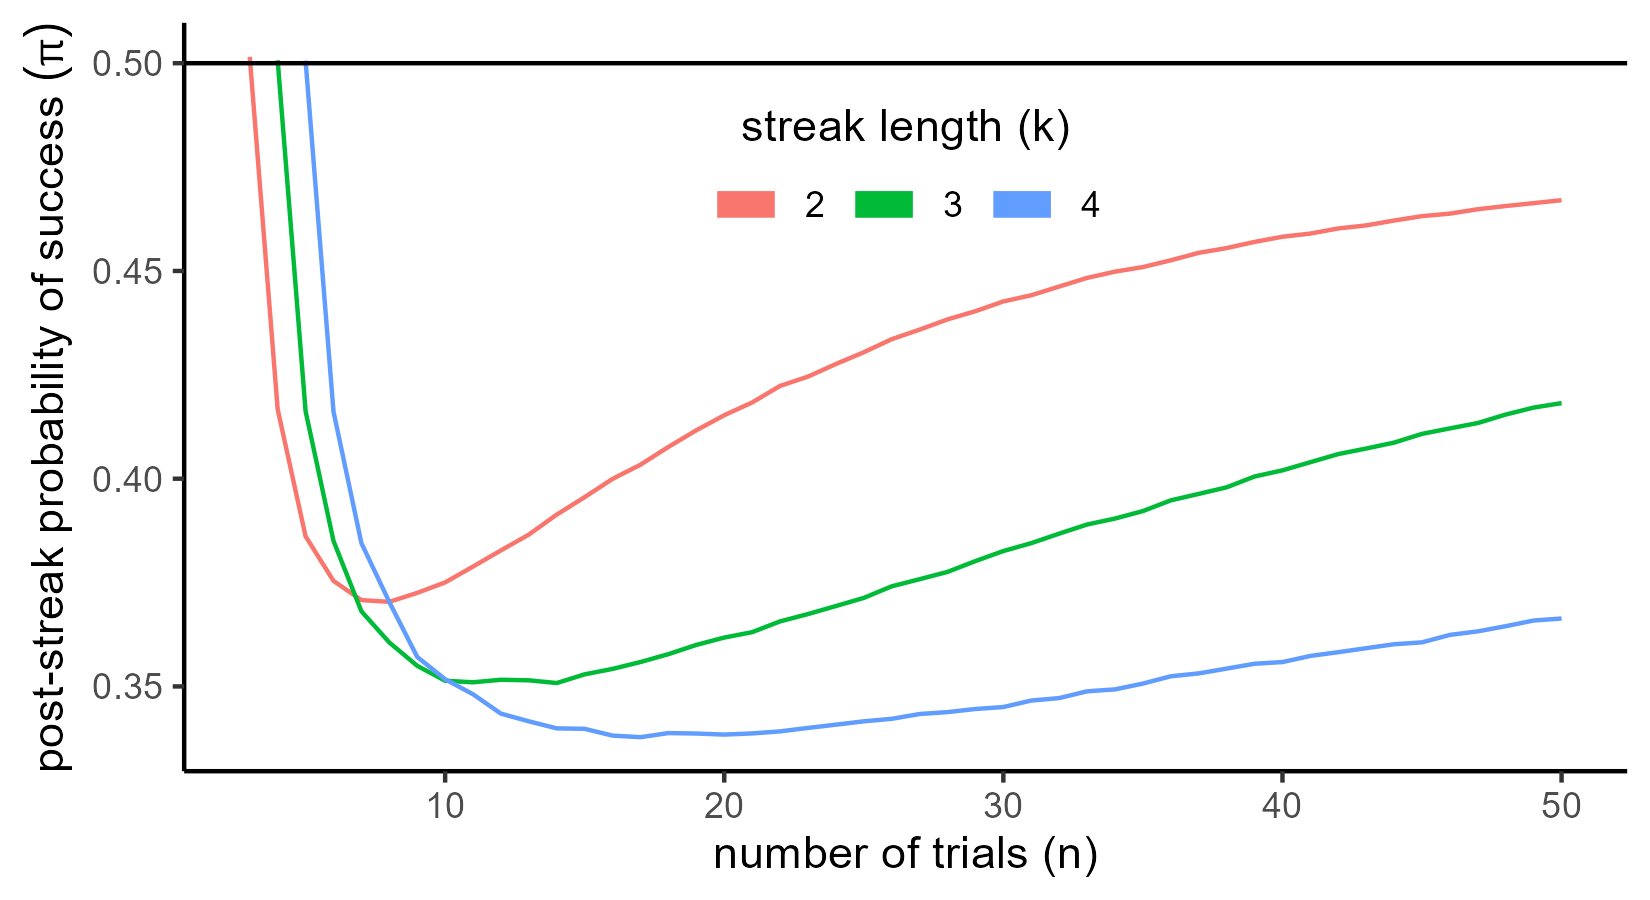
\includegraphics{images/pwkr_ms.png}
\caption{The expected value of the proportion of successes on trials that immediately follow $k$ consecutive successes, $E[\hat{\Pi}_k(\mathbf{X}) | I_k(\mathbf{X}) \neq \emptyset]$, for Bernoulli trial success $\pi = 0.5$ and streak lengths $k \in [2, 3, 4]$, as a function of the total number of trials $n.$}
\end{figure}

My context is fundamentally different from that of GVT and MS, both of
whom focus on longitudinal data in controlled settings. GVT also perform
statistical tests on shots from players in live games,
i.e.~``observational'' data, but they note that their findings are
likely affected player shot selection in the face of defensive strategy
by the opposing team. The number of trials is fixed in their
experimental designs, but in CoD SnD, the number of rounds played is
determined as a function of the max number of possible rounds (\(s\))
and whether or not the team wins the series, as shown in Equation
\ref{eq:pwr}. The Bernoulli trial success probability, i.e.~a round win
in CoD SnD, is not independent of the opponent.

Consequently, a statistical test of the difference in \(\hat{P}^{w|kr}\)
and \(\hat{P}^{\ell|kr}\), as performed by GVT and MS to evaluate their
respective hypothesis regarding
\(E[\hat{P}_k(\mathbf{X}) | I_k(\mathbf{X}) \neq \emptyset]\) (Theorem
1), is not appropriate.

Let us consider another form of the expected proportion of rounds won
immediately after a streak of \(k\) round wins in a best-of-\(s\) series
given the length of the series (\(r\) rounds), the ``hindsight''
proportion \(\hat{P}^{w|kr}_0\). The Bernoulli round win probability
underlying \(\hat{P}^{w|kr}_0\) is

\begin{equation}\protect\hypertarget{eq:pwkr}{}{
p_0^{w|kr} = p_0(\text{win | k, r})=\{
\begin{array}{cl}
\frac{m - k}{i - k}, & \text{team wins series} \\
\frac{s - m - k}{i - k}, & \text{team loses series}
\end{array}.
}
\label{eq:pwkr}
\end{equation}

A binomial test for the expected proportion of round wins following
streaks of \(k\) round wins in a series lasting \(r\) rounds,
\(\hat{P}^{w|kr}_0\), assuming \(p^{w|kr}_0\) as the probability of
success, can be used to verify that \(\hat{P}^{w|kr}_0\) is reasonable
as to use as a baseline with which to compare \(\hat{P}^{w|kr}_{MS}\).
If the binomial test shows that we cannot reject the null hypothesis
that the expected \(\hat{P}^{w|kr}_0\) is different from the observed
proportion \(P^{w|kr}\).

A proportion test of \(\hat{P}^{w|kr}_0\) and \(\hat{P}^{w|kr}_{MS}\)
can tell us whether the momentum exists in CoD SnD. A null result means
we cannot say that there is a difference between the hindsight expected
proportion \(\hat{P}^{w|kr}_0\) and the expected proportion adjusted for
streak-selection bias, \(\hat{P}^{w|kr}_0\).

\hypertarget{results}{%
\section{Results}\label{results}}

First, I investigate the constant probability assumption and the
distribution of rounds played in a series. Chance's (2020) work is
closely related to mine, and, in fact, provides a guide for this
investigation. Afterwards, I investigate post-streak win rates and the
context of momentum, leveraging MS's (2018) framework for streak
selection bias.

\hypertarget{sec:results-rounds-played}{%
\subsection{Distribution of rounds
played}\label{sec:results-rounds-played}}

Using Equation \ref{eq:chi-squ}, I find that \(\chi^2 = 16.0\) (p-value
of 0.0068) for the naive constant round win probability
\(\phi_0 = 0.5\). Thus, I can comfortably reject the constant
probability null hypothesis for \(\phi_0 = 0.5\), even at a confidence
level of \(\alpha = 0.01\).

Table \ref{tbl:cod-prob-series-lasting-r-rounds} shows the expected
series lasting \(r\) rounds, \(\hat{\Phi}_0(r)\) (under the assumption
\(\phi_0 = 0.5\)), for \(s = 11\), along with the observed proportions,
\(\Phi(r)\), in CoD SnD.

\begin{longtable}{rrrr}
\caption{The expected proportion of series lasting $r$ rounds ($\hat{\Phi}_0(r)$) in a best-of-11 format, wehre $r \in R = [6, 7, 8, 9, 10, 11]$ under the assumption that each team has a constant round win probability $\phi_0 = 0.5$. The observed frequencies for CoD SnD are shown as a count $N(r)$ and as a proportion $\Phi(r)$ of all series ($\sum^R N(r)$).}\label{tbl:cod-prob-series-lasting-r-rounds} \\
\toprule
$r$ & $\hat{\Phi}_0(r)$ & $\Phi(r)$ & $N(r)$ \\ 
\midrule
6 & $3.1\%$ & $4.7\%$ & 40 \\ 
7 & $9.4\%$ & $11.9\%$ & 101 \\ 
8 & $16.4\%$ & $16.5\%$ & 141 \\ 
9 & $21.9\%$ & $21.7\%$ & 185 \\ 
10 & $24.6\%$ & $21.5\%$ & 183 \\ 
11 & $24.6\%$ & $23.7\%$ & 202 \\ 
\bottomrule
\end{longtable}

Table \ref{tbl:mosteller-methods-results} shows the alternate values for
the constant round win probability that I find when applying the three
methods suggested by Mosteller (1952). Each is approximately or equal to
0.575, and, when applying Equation \ref{eq:chi-squ}, each results in a
\(\chi^2\) value for which I cannot reject the constant probability null
hypothesis.

\begin{longtable}[]{@{}lrr@{}}
\caption{Alternate estimates of the constant probability ($\phi$) for winning a given round in a CoD SnD, applying the three methods suggested by Mosteller (1952), in addition to the naive ($\phi_0 = 0.5$).}\label{tbl:mosteller-methods-results} \\
\toprule()
Method & $\phi$ & $\chi^2$ (p-value) \\
\midrule()
\endfirsthead
\toprule()
Method & $\phi(r)$ & $\chi^2$ (p-value) \\
\midrule()
\endhead
0. Naive & 0.5000 & 16.0 (\textless=0.01) \\
1. Method of moments & 0.5725 & 3.6 (0.6) \\
2. Maximum likelihood & 0.5750 & 3.5 (0.62) \\
3. Minimum ($\chi^2$) & 0.5775 & 3.5 (0.62) \\
\bottomrule()
\end{longtable}

Table \ref{tbl:expected-series-lengths-alternative-ps} shows the new
\(\hat{\Phi}(r)\) when re-applying Equation \ref{eq:series-length} for
the maximum likelihood estimate \(\phi_2 = 0.575\), resulting in a new
set of expected proportions of series lasting \(r\) rounds
\(\hat{\Phi}_2(r)\).\footnote{The method of moments and minimum
  \(\chi^2\) estimates for \(\phi\) are omitted simply because the
  results would be nearly identical to those for the maximum likelihood
  estimate of \(\phi\) (since they are all \(\approx 0.575\)).} I
observe that \(\hat{\Phi}_2(r)\) is larger than \(\hat{\Phi}_0(r)\) for
\(r \in [6, 7]\), more closely matching \(\Phi(r)\). \(\hat{\Phi}_2(r)\)
is also closer to the observed \(\Phi(r)\) for \(r \in [9, 10]\),
although not for \(r \in [8, 11]\).

\begin{longtable}[]{@{}rrrr@{}}
\caption{The observed proportion of series $\Phi(r)$ ending in $r$ rounds in CoD SnD's best-of-11 format, compared to the expected proportion $\hat{\Phi}_0(r)$ the naive assumption $\phi_0 = 0.5$ and the expected proportion $\hat{\Phi}_2(r)$ under the maximum likelihood estimate $\phi_2 = 0.575$ for constant round win probability.}\label{tbl:expected-series-lengths-alternative-ps} \\
\toprule()
$r$ & $\hat{\Phi}_0(r)$ = 0.5 & $\hat{\Phi}_2(r)$ = 0.575 & $\Phi(r)$ \\
\midrule()
\endhead
6 & 3.1\% & 4.2\% & 4.7\% \\
7 & 9.4\% & 11.2\% & 11.9\% \\
8 & 16.4\% & 17.8\% & 16.5\% \\
9 & 21.9\% & 21.8\% & 21.7\% \\
10 & 24.6\% & 23.0\% & 21.5\% \\
11 & 24.6\% & 22.0\% & 23.7\% \\
\bottomrule()
\end{longtable}

Observing that \(\hat{\Phi}_2(r)\) reasonably matches \(\Phi(r)\)
(especially in comparison to \(\hat{\Phi}_0(r)\)), along with the null
hypothesis rejection shown in Table \ref{tbl:mosteller-methods-results},
it is fair to conclude that the constant round win probability
assumption can be valid in CoD SnD series with the appropriate choice of
\(\phi\) (\(\approx 0.575\)).

\hypertarget{sec:results-momentum}{%
\subsection{Momentum}\label{sec:results-momentum}}

Given that people typically perceive streaks as beginning after the
third success (or failure) at minimum (Carlson and Shu 2007), I focus on
streaks of three round wins.\footnote{Three happens to also be a
  reasonable number for series that lasts at maximum 11 rounds.} Table
\ref{tbl:cod-pw3r-pl3r} shows \(P^{w,kr}\) and \(P^{l,kr}\) for round
win rate and loss rate following \(k = 3\) round win streaks
respectively.

First,

\begin{longtable}{rrrrrrr}
\caption{Observed count and proportion of round wins immediately following round win streak of $k=3$, $N^{w|kr}$ and $P^{w|kr}$ respectively, in series lasting $r$ rounds. Additionally, notional expected proportion, $\hat{P}^{w|kr}_0$ and binomial test p-value, assuming notional round probability $p^{w|kr}$ and using observed counts; MS expected proportion $\hat{P}^{w|kr}_{MS}$; and $\hat{D}^{w|kr} = \hat{P}^{w|kr}_{MS} - \hat{P}^{w|kr}_0$ and proportion test p-value. Fields presented in groups, split by whether the team won the round immediately following the 3-round win streak, and whether the team won the series. The post-streak loss analogues are presented as $N^{\ell|kr}$, $P^{\ell|kr}$, $\hat{P}^{\ell|kr}_0$, $\hat{P}^{\ell|kr}_{MS}$, and $\hat{D}^{\ell|kr}$.}
\label{tbl:cod-pw3r-pl3r} \\
\toprule
\multicolumn{6}{c}{\text{win series, win after 3-round win streak}} \\
\midrule
$r$ & $N^{w|kr}$ & $P^{w|kr}$ & $\hat{P}^{w|kr}_0$ ($p$-value) & $\hat{P}^{w|kr}_{MS}$ & $\hat{D}^{w|kr}$ ($p$-value) \\ 
\midrule
7 & 209 & 74.6\% & 75.0\% (0.58) & 75.7\% & -0.7\% (0.94) \\ 
8 & 209 & 62.2\% & 60.0\% (0.28) & 61.9\% & -1.9\% (1.00) \\ 
9 & 193 & 51.8\% & 50.0\% (0.33) & 52.7\% & -2.7\% (0.97) \\ 
10 & 151 & 43.7\% & 42.9\% (0.45) & 44.7\% & -1.8\% (0.94) \\ 
11 & 150 & 40.0\% & 37.5\% (0.29) & 38.8\% & -1.3\% (1.00) \\ 
\toprule
\toprule
\multicolumn{6}{c}{\text{lose series, win after 3-round win streak}} \\
\midrule
$r$ & $N^{w|kr}$ & $P^{w|kr}$ & $\hat{P}^{w|kr}_0$ ($p$-value) & $\hat{P}^{w|kr}_{MS}$ & $\hat{D}^{w|kr}$ ($p$-value) \\ 
\midrule
10 & 60 & 13.3\% & 14.3\% (0.64) & 26.7\% & -12.4\% (1.00) \\ 
11 & 129 & 24.0\% & 25.0\% (0.63) & 30.8\% & -5.8\% (0.98) \\ 
\toprule
\toprule
\multicolumn{6}{c}{\text{win series, lose after 3-round win streak}} \\
\midrule
$r$ & $N^{\ell|kr}$ & $P^{\ell|kr}$ & $\hat{P}^{\ell|kr}_0$ ($p$-value) & $\hat{P}^{\ell|kr}_{MS}$ & $\hat{D}^{\ell|kr}$ ($p$-value) \\ 
\midrule
7 & 209 & 25.4\% & 25.0\% (0.48) & 6.4\% & 18.6\% (0.98) \\ 
8 & 209 & 37.8\% & 40.0\% (0.76) & 14.7\% & 25.3\% (0.96) \\ 
9 & 193 & 48.2\% & 50.0\% (0.72) & 22.2\% & 27.8\% (0.97) \\ 
10 & 151 & 56.3\% & 57.1\% (0.62) & 26.7\% & 30.5\% (0.99) \\ 
11 & 150 & 60.0\% & 62.5\% (0.76) & 30.8\% & 31.7\% (0.95) \\ 
\toprule
\toprule
\multicolumn{6}{c}{\text{lose series, lose after 3-round win streak}} \\
\midrule
$r$ & $N^{\ell|kr}$ & $P^{\ell|kr}$ & $\hat{P}^{\ell|kr}_0$ ($p$-value) & $\hat{P}^{\ell|kr}_{MS}$ & $\hat{D}^{\ell|kr}$ ($p$-value) \\ 
\midrule
10 & 60 & 86.7\% & 85.7\% (0.51) & 44.7\% & 41.1\% (1.00) \\ 
11 & 129 & 76.0\% & 75.0\% (0.45) & 38.8\% & 36.2\% (0.95) \\ 
\bottomrule
\end{longtable}

\hypertarget{references}{%
\section*{References}\label{references}}
\addcontentsline{toc}{section}{References}

\hypertarget{refs}{}
\begin{CSLReferences}{1}{0}
\leavevmode\vadjust pre{\hypertarget{ref-ayton2004}{}}%
Ayton, Peter, and Ilan Fischer. 2004. {``The Hot Hand Fallacy and the
Gambler{'}s Fallacy: Two Faces of Subjective Randomness?''} \emph{Memory
\& Cognition} 32 (8): 13691378.

\leavevmode\vadjust pre{\hypertarget{ref-carlson2007}{}}%
Carlson, Kurt A., and Suzanne B. Shu. 2007. {``The Rule of Three: How
the Third Event Signals the Emergence of a Streak.''}
\emph{Organizational Behavior and Human Decision Processes} 104 (1):
113121.

\leavevmode\vadjust pre{\hypertarget{ref-chance2020}{}}%
Chance, Don. 2020. {``Conditional Probability and the Length of a
Championship Series in Baseball, Basketball, and Hockey.''}
\emph{Journal of Sports Analytics} 6 (2): 111--27.
\url{https://doi.org/10.3233/JSA-200422}.

\leavevmode\vadjust pre{\hypertarget{ref-derover2021}{}}%
DeRover, DeMars. 2021. {``Round Win Probabilities Based on Who's Alive +
Time.''}
\url{https://www.reddit.com/r/VALORANT/comments/n3lpoo/round_win_probabilities_based_on_whos_alive_time/}.

\leavevmode\vadjust pre{\hypertarget{ref-gilovich1985}{}}%
Gilovich, Thomas, Robert Vallone, and Amos Tversky. 1985. {``The Hot
Hand in Basketball: On the Misperception of Random Sequences.''}
\emph{Cognitive Psychology} 17 (3): 295314.

\leavevmode\vadjust pre{\hypertarget{ref-miller2018}{}}%
Miller, Joshua B., and Adam Sanjurjo. 2018. {``Surprised by the Hot Hand
Fallacy? A Truth in the Law of Small Numbers.''} \emph{Econometrica} 86
(6): 20192047.

\leavevmode\vadjust pre{\hypertarget{ref-mosteller1952}{}}%
Mosteller, Frederick. 1952. {``The World Series Competition.''}
\emph{Journal of the American Statistical Association} 47 (259): 355380.

\leavevmode\vadjust pre{\hypertarget{ref-steeger2021}{}}%
Steeger, Gregory M., Johnathon L. Dulin, and Gerardo O. Gonzalez. 2021.
{``Winning and Losing Streaks in the National Hockey League: Are Teams
Experiencing Momentum or Are Games a Sequence of Random Events?''}
\emph{Journal of Quantitative Analysis in Sports} 17 (3): 155170.

\leavevmode\vadjust pre{\hypertarget{ref-vafa2017}{}}%
Vafa, Keyon. 2017. {``Is the Hot Hand Fallacy a Fallacy?''}
\url{https://keyonvafa.github.io/hot-hand/}.

\leavevmode\vadjust pre{\hypertarget{ref-xenopoulos2022}{}}%
Xenopoulos, Peter, William Robert Freeman, and Claudio Silva. 2022.
{``Analyzing the Differences Between Professional and Amateur Esports
Through Win Probability.''} In, 34183427.

\end{CSLReferences}

\bibliographystyle{unsrt}
\bibliography{references.bib}


\end{document}
